% This is samplepaper.tex, a sample chapter demonstrating the
% LLNCS macro package for Springer Computer Science proceedings;
% Version 2.20 of 2017/10/04
%
\documentclass[runningheads]{llncs}
%
\usepackage{graphicx}
\usepackage{color}
\usepackage{amsmath}
\usepackage{amssymb}
\usepackage{bcprules, proof}
\usepackage{fancybox}
\usepackage{mathtools}
\usepackage{float}
\usepackage{xparse}
\usepackage{lscape}
\usepackage{mdframed}
\usepackage{xspace}

% Used for displaying a sample figure. If possible, figure files should
% be included in EPS format.
%
% If you use the hyperref package, please uncomment the following line
% to display URLs in blue roman font according to Springer's eBook style:
% \renewcommand\UrlFont{\color{blue}\rmfamily}

\newcommand{\red}[1]{\textcolor{red}{#1 }}
\newcommand{\blue}[1]{\textcolor{blue}{#1 }}

\newcommand{\LTP}{$\lambda^{\triangleright\%}$\xspace}
\newcommand{\LMD}{$\lambda^{\textrm{MD}}$\xspace}
\newcommand{\LLF}{$\lambda\textrm{LF}$\xspace}

\newcommand{\G}{\Gamma}
\newcommand{\D}{\Delta}
\newcommand{\V}{\vdash_\Sigma}
\newcommand{\VT}{\vdash\hspace{-.50em}\raisebox{0.28em}{\tiny{$\TB$}}}
\newcommand{\iskind}{\text{\ kind}}
\newcommand{\TW}{\triangleright}
\newcommand{\TWL}{\triangleleft}
\newcommand{\F}{\forall}
\newcommand{\TB}{\blacktriangleright}
\newcommand{\TBL}{\blacktriangleleft}
\newcommand{\E}{\equiv}
\newcommand{\FV}{\text{FV}}
\newcommand{\FTV}{\text{FSV}}

\newcommand{\WStar}{\textsc{W-Star}}
\newcommand{\WAbs}{\textsc{W-Abs}}
\newcommand{\WCsp}{\textsc{W-Csp}}
\newcommand{\WApp}{\textsc{W-App}}
\newcommand{\WTW}{\textsc{W-$\TW$}}

\newcommand{\KVar}{\textsc{K-Var}}
\newcommand{\KAbs}{\textsc{K-Abs}}
\newcommand{\KApp}{\textsc{K-App}}
\newcommand{\KConv}{\textsc{K-Conv}}
\newcommand{\KTW}{\textsc{K-$\TW$}}
\newcommand{\KTWL}{\textsc{K-$\TWL$}}
\newcommand{\KGen}{\textsc{K-Gen}}
\newcommand{\KCsp}{\textsc{K-Csp}}

\newcommand{\TConst}{\textsc{T-Const}}
\newcommand{\TVar}{\textsc{T-Var}}
\newcommand{\TAbs}{\textsc{T-Abs}}
\newcommand{\TApp}{\textsc{T-App}}
\newcommand{\TConv}{\textsc{T-Conv}}
\newcommand{\TTB}{\textsc{T-$\TB$}}
\newcommand{\TTBL}{\textsc{T-$\TBL$}}
\newcommand{\TGen}{\textsc{T-Gen}}
\newcommand{\TIns}{\textsc{T-Ins}}
\newcommand{\TCsp}{\textsc{T-Csp}}

\newcommand{\QKAbs}{\textsc{QK-Abs}}
\newcommand{\QKCsp}{\textsc{QK-Csp}}
\newcommand{\QKRefl}{\textsc{QK-Refl}}
\newcommand{\QKSym}{\textsc{QK-Sym}}
\newcommand{\QKTrans}{\textsc{QK-Trans}}

\newcommand{\QTAbs}{\textsc{QT-Abs}}
\newcommand{\QTApp}{\textsc{QT-App}}
\newcommand{\QTTW}{\textsc{QT-$\TW$}}
\newcommand{\QTGen}{\textsc{QT-Gen}}
\newcommand{\QTCsp}{\textsc{QT-Csp}}
\newcommand{\QTRefl}{\textsc{QT-Refl}}
\newcommand{\QTSym}{\textsc{QT-Sym}}
\newcommand{\QTTrans}{\textsc{QT-Trans}}

\newcommand{\QAbs}{\textsc{Q-Abs}}
\newcommand{\QApp}{\textsc{Q-App}}
\newcommand{\QTB}{\textsc{Q-$\TB$}}
\newcommand{\QTBL}{\textsc{Q-$\TBL$}}
\newcommand{\QGen}{\textsc{Q-Gen}}
\newcommand{\QIns}{\textsc{Q-Ins}}
\newcommand{\QCsp}{\textsc{Q-Csp}}
\newcommand{\QRefl}{\textsc{Q-Refl}}
\newcommand{\QSym}{\textsc{Q-Sym}}
\newcommand{\QTrans}{\textsc{Q-Trans}}
\newcommand{\QBeta}{\textsc{Q-$\beta$}}
\newcommand{\QEta}{\textsc{Q-$\eta$}}
\newcommand{\QTBLTB}{\textsc{Q-$\TBL\TB$}}
\newcommand{\QLambda}{\textsc{Q-$\Lambda$}}
\newcommand{\QPercent}{\textsc{Q-\%}}

\newcommand{\ID}[1]{\infer[]{#1}{\vdots}}
\newcommand{\MD}[1]{\mathcal{D}_#1}

\newcommand{\I}{\textrm{Int}}
\newcommand{\B}{\textrm{Bool}}
\newcommand{\M}{\textrm{Mat}}

\begin{document}
%
\title{A Dependently Typed Multi-Stage Calculus\thanks{Supported by organization x.}}
%
%\titlerunning{Abbreviated paper title}
% If the paper title is too long for the running head, you can set
% an abbreviated paper title here
%
\author{Akira Kawata\inst{1} \and
    Atsushi Igarashi\inst{2}\orcidID{0000-0002-5143-9764}}
%
\authorrunning{A. Kawata, A. Igarashi}
% First names are abbreviated in the running head.
% If there are more than two authors, 'et al.' is used.
%
\institute{Graduate School of Informatics, Kyoto University, Kyoto, Japan\\
    \email{akira@fos.kuis.kyoto-u.ac.jp} \and
    \email{igarashi@kuis.kyoto-u.ac.jp}
}
%
\maketitle              % typeset the header of the contribution
%
\begin{abstract}

    We develop yet another typed multi-stage calculus \LMD.
    It extends Hanada and Igarashi's \LTP with dependent types.
    A multi-stage calculus enables us to generate and execute codes at runtime.
    It can improve the performance of programs by generating optimized codes for given inputs.
    Dependent types are types dependent on values. 
    A vector with its length is a famous example of dependent types and it enables us to omit boundary checking.
    In this paper, we design \LMD by introducing dependent type into $\lambda^{\TW\%}$.
    You can make more efficient programs from existing dependent typed programs with \LMD.
    \LMD has a simple, substitution-based full-reduction semantics and enjoys basic properties of subject reduction, confluence, and strong normalization, and progress.
    It also includes an evaluation context which satisfies unique decomposition.
    The main technical points of this paper are how to deal with Cross Stage Persistence of multi-stage calculuses which allows using a value in quoted code in a dependent type system.
    Especially, the way of handling CSP in equivalence rules of dependent types wasn't clear.
    In this paper, we give reasonable equivalence rules to handle them.
    
    \keywords{Multistage programming \and Dependent type}
\end{abstract}

\blue{181 words. The abstract should briefly summarize the contents of the paper in 150--250 words.}
\blue{コードとかはボールドを使ったほうが良いかもしれない。}
\red{Suspicious senetences are colored red.}
%
%
%
\red{Multistage Programming と Multistage Calculus をどう使い分けるか?}

\section{Introduction}

\subsection{Multistage Programming}

% \subsubsection{多段階計算とは何か?}

Multistage programming enables us to generate and run fragments of code at runtime.
MetaOCaml\cite{oleg2014} provide features for multistage programming, which are brackets, escape, and run.
Brackets, written \verb|.< e >.| in MetaOCaml, makes a code value from \verb|e|.
Run, written \verb| run e | in MetaOCaml, runs a code value of \verb|e| and restore \verb|e|.
Escape, written \verb| .~ e | in MetaOCaml, expands a code value of \verb|e|.
Unlike run, escape is supposed to use in a fragment of code, that is, escape cannot be used as an alternative of run.
For example, the following MetaOCaml expression

\begin{verbatim}
        let plusone = .< fun x -> x + 1 >. in .< .~plusone 2 >.
\end{verbatim}
evaluates to \verb|.< (fun x -> x + 1) 2 >.|. We can get the result with run.
\begin{verbatim}
        run (let plusone = .< fun x -> x + 1 >. in .< .~plusone 2 >.)
\end{verbatim}
is reduced to 3.

% \subsubsection{CSPに関する補足説明}

Cross-stage Persistence (CSP) is another primitive of multistage programming, which enable us to embed computed values into a code value.
This is an example of CSP.
\begin{verbatim}
        let plusone = fun x -> x + 1 in
        let y = plusone 2 in  .< y >.
\end{verbatim}
This program evaluates to \verb|.< 3 >.| not  \verb|.< plusone 2 >.|.
This is because the variable \verb|y| is introduced into a code fragment using CSP.
Therefore, the variable \verb|y| is embedded after it was calculated.
CSP is very important when we write practical programs 
because CSP enables us to use library functions in code fragments as in \verb|.<List.combine [1;2] ['a';'b']>.|.

% \subsubsection{多段階計算のメリットをべき乗の例を用いて説明する}

The main application of multistage calculi is program optimization.
A famous example is power functions.
Usual power functions take two arguments, which are the base and the exponent.
We can make a specialized power function for given exponents with multistage programming and 
optimize them by unrolling a loop in functions for given exponents.
The optimized power function for the exponent of \verb|3| looks like \verb|power3 = fun x -> x * x * x|.
\verb|power3| is faster than ordinary \verb|power| function because it contains no loop.
Multistage programming can optimize functions which take more than two arguments 
by generating a code fragment optimized to a given argument.

% \subsubsection{ベクトル計算も高速化できる}

Multistage programming can also optimize vector calculation.
For example, \verb|vadd| function, which takes two vectors and return the sum of them,
is implemented with a loop in many cases.
We can unroll \verb|vadd| function for a given vector length and optimize it with multistage programming.
\red{MetaOCamlで書いた長さ付きベクトルの例?}

% \subsubsection{生成した行列計算のコードは特定のサイズに特化しており、他のサイズでは使えない。
% このため、間違って組み合わせると容易にエラーを引き起こす。既存の型システムではこのエラーを防止できない}

However, there is a sever problem in functions which are optimized by multistage programming.
Although unrolled \verb|vadd| function is optimized, we cannot use it for different vector length.
For example, when you optimize for the length of 5, you shouldn't use it for vectors of 3 lengths.
Otherwise, we will get a Segmentation Fault error.
This problem is serious but existing type systems for multistage calculi cannot prevent it.

% We call this problem \red{Specialized Code Problem}.

\subsection{Dependent Types}

% \subsubsection{依存型とは何か?}

Dependent types are types which is dependent on values.
We can use dependent types for securer programming.
For example, we can realize vectors with their sizes with them.
\begin{verbatim}
        Vector :: Int -> *
\end{verbatim}
\verb|Vector| is a type constor which takes the length of vectors, that is, 
\verb|Vector 3| is a type for vectors whose lengths are 3.
If \verb|vadd| function has the type of \verb|Vector n -> Vector n -> Vector n|,
we can confirm the two arguments of \verb|vadd| function has the same length.
\red{secure programming? finer grained typing? とか}

\subsection{Multistage Programming with Dependent Types}
\red{このsubsectionは短いので上とくっつけてもいいかもしれない}

% \subsubsection{「生成した行列計算のコードは特定のサイズに特化しており、他のサイズでは使えない。
% このため、間違って組み合わせると容易にエラーを引き起こす。」問題を依存型で解決する。}

As we pointed out in the above section,
functions optimized with multistage programming can take only restricted values as arguments.
When you optimize \verb|vadd| function for the length of 5, you should it only for 5 length vectors.
We introduce dependent types into a multistage calculus
so that the type system can guarantee optimized functions are used properly.

In this paper, we design new multistage calculus \LMD by 
merging dependent types into existing multistage calculus \LTP\cite{Hanada2014}.
\LMD is multistage calculus which contains dependent types.
\LMD makes multistage programming more safer with the power of dependent types.

\subsection{Organization of the Paper}

The organization of this paper is the following.
Section 2 gives an informal overview of \LMD.
Section 3 defines the syntax, type system, full reduction, evaluation contexts of \LMD.
Section 4 shows the properties of \LMD including Unique Decomposition.
Section 5 discusses future works.
Finally, Section 6 discusses related works.

\section{Informal Overview of \LMD}

We designed \LMD, a multistage calculus with dependent type.
\LMD is based on \LTP\cite{Hanada2014} by Hanada and Igarashi, which is a multistage calculus with CSP and
we introduced dependent types based on \LTP\cite{attapl}.
In this section, we check \LMD informally after checking \LTP and \LLF which are the basis of \LMD.

\red{\LTP\cite{Hanada2014}が頻発するが同一論文の複数回引用に何かルールはあるのか?}
\subsection{\LTP}

% quote and unquote

\LTP\cite{Hanada2014} is a multistage calculus with CSP by Hanada and Igarashi.
In \LTP, brackets and escape are written $\TB_\alpha M$ and $\TBL_\alpha M$, respectively.
The type of $\TB_\alpha M$ is $\TW_\alpha \tau$ if $M$ has type $\tau$.
The type of $\TBL_\alpha M$ is $\tau$ if $M$ has $\TW_\alpha \tau$.
% Please notice that if $\TBL_\alpha M$ is well-typed, $M$ has a code type from the typing rule of \LTP.
In addition to normal $\beta$-reduction, there is a reduction rule for brackets and escape.
\begin{align*}
    \TBL_\alpha (\TB_\alpha M) \longrightarrow M
\end{align*}
It means escape cancels brackets.
% This reduction is called $\longrightarrow_\Lambda$ in \LMD.
% \red{この文はここに来るべきなのか? LTPの説明ではないが}

% transition variable

The subscript $\alpha$ in $\TB_\alpha M$ is a \textit{transition variable}.
It is used to show the thickness of brackets.
For example, $\TB_\alpha (\lambda x:\I.x+10)$ is the fragment of code which becomes $(\lambda x:\I.x+10)$ after it was run once and
$\TB_\alpha \TB_\beta (\lambda x:\I.x+10)$ becomes $(\lambda x:\I.x+10)$ after it was run it twice.
\red{run twiceは表現が微妙}

% transition

A sequence of transition variables is a \textit{transition}.
In \LTP, all judgment has a transition.
Especially, terms without quoting exist at the empty transition which is represented by $\epsilon$.
For example, $(\lambda x:\I.x)\ (1+2)$ is at $\epsilon$ transition and 
$\TB_\alpha (\lambda x:\I.x)$ is at $\alpha$ transition.

% transition in typing rules

\red{LTPに合わせて$\vdash^A$を使うべきか? それともLMDに合わせて$\vdash @ A$を使うべきか?}

A type judgement of \LTP is of the form $\G \vdash M : \tau @ A$.
Transition $A$ means in which transition $M$ exists.
Therefore, transitions appear in typing rules, too.
\begin{center}
    \infrule{\G\vdash M:\tau @{A\alpha}}{\G\vdash \TB_{\alpha}M:\TW_{\alpha}\tau @A}{\TTB} \andalso
    \infrule{\G\vdash M:\TW_{\alpha}\tau @A}{\G\vdash \TBL_{\alpha}M:\tau @{A\alpha}}{\TTBL}
\end{center}
\TTB, corresponding to quoting, means 
if $M$ is typed $\tau$ at transition $A\alpha$ then $\TB_{\alpha}M$, quoted $M$, is typed $\TW_{\alpha}\tau$ at $A$.
\TTBL is converse of \TTB.

% transition abstraction and application

There are abstractions for transition variables and applications for transition abstraction in \LTP.
They look like $\Lambda\alpha.M$ and $M\ A$, respectively.
A transition abstraction binds a transition variable in a term.
For example, all $\alpha$ in $\Lambda\alpha.(\TB_\alpha (\lambda x:\I.x))$ are bound.
It is only natural there is a rule for transition application in \LTP.
The rule is the following.

\begin{align*}
    (\Lambda\alpha.M)\ A \longrightarrow M[\alpha\mapsto A]
\end{align*}

For example, $\Lambda\alpha.(\TB_\alpha (\lambda x:\I.x))\ (\beta\gamma)$ reduces to $\TB_{\beta\gamma} (\lambda x:\I.x)$.
Although we can apply any transition to a transition abstraction in \LTP,
we restrict the transitions only to $\epsilon$ transition in \LMD to simplify the system.
\red{この文はここに来るべきなのか? LTPの説明ではないが}

% transition-related symbols disappear when the empty transition is substituted.

Another important rule about a transition variable is 
that a transition variable related symbol disappears when the empty transition is substituted to the transition variable.
For example, $(\TB_\epsilon (\lambda x:\I.x))$ is equivalent to $(\lambda x:\I.x)$.
This rule is applied all transition variable related symbols: $\TB_\alpha, \TBL_\alpha$, and $\%_\alpha$.

% Run
The main purpose of transition abstractions and transition applications are to represent {\bf{run}} operator.
In multistage calculus, {\bf{run}} is a very important operator.
It changes quoted code to the original code.
{\bf{run}} is realized with application of the empty transition $\epsilon$.
For example, $\Lambda\alpha.(\TB_\alpha (\lambda x:\I.x))\ \epsilon$ becomes $\lambda x:\I.x$
because $\TB_\epsilon$ is disappeared.

% CSP
CSP, cross-stage persistence, is an important feature of multistage calculus.
It enables us to embed value at an outer transition into an inner transition.
\red{inner / outer は適切か?}
$\%$ is dedicated to CSP in \LTP.
For example, $\lambda a:\I.\Lambda\alpha.(\TB_\alpha (\lambda x:\I.x+\%_\alpha a))$

% Omitting Residualization

There is another important function called program residualization in \LTP.
It means that a generated code can be dumped into a file.
We can load the dumped file and run it.
The difficulty arises when program residualization is used with CSP.
Transition variables are classified into two kinds in \LTP in order to deal with this difficulty.

\subsection{\LLF}

% \LLF
\LLF is a simple system of dependent types introduced in \cite{attapl}.
\red{system / type system / calculus?}
It is based on Edinburgh LF\cite{harper1993framework}.
Therefore, all constants and base types are declared in the signature.
The \LLF type theory generalizes simply typed lambda calculus
by replacing the function type $\tau\to\sigma$ with the dependent product type $\Pi x:\tau.\sigma$.

% Kind, Well-formed kind
In addition to ordinary typing rules like simply typed lambda calculus,
there are kinding rules, well-formed kinding rules, term equivalence rules, type equivalence rules, and kind equivalence rules in \LLF.
Kinding rules and well-formed kinding rules are 
introduced in order to prohibit making illegal types such as $\textrm{Vect}\ \textrm{Bool}$.
For a well-formed type $\tau$, $\G \vdash \tau :: K$ means that $\tau$ has a kind $K$ under the environment $\G$ and 
for a well-formed kind $K$, $\G \vdash K$ means that $K$ is a well-formed kind under an environment $\G$.

% Type Equality
Type equality rules are needed because the type equivalence is not obvious unlike simply typed lambda calculus.
For example, $\textrm{Vect}\ 7$ should be equivalent to $\textrm{Vect}\ (3+4)$
but they are not equivalent seemingly. Thus, we must define equivalence rules.
In \LLF, equivalence is expressed with a symbol of $\E$.
$\G \vdash M \E N$ means a term $M$ and a term $N$ are equivalent under the environment $\G$.
$\G \vdash \tau \E \sigma$ means a type $\tau$ and a type $\sigma$ are equivalent under the environment $\G$.
$\G \vdash K \E J$ means a kind $K$ and a kind $J$ are equivalent under the environment $\G$.

\subsection{Extending \LTP with Dependent Types}

Next, we develop \LMD by extending \LTP with \LLF-like dependent types.
From here, we use the word "stage" instead of "transition" 
because we develop a multi-stage calculus, not a multi-transition calculus.
\red{stageのほうが言葉としてふさわしいと言いたい}
There are three technical points in the extension from \LTP to \LMD.

\red{, which is called a \textit{stage variable} in \LMD.}
\red{ which is called a stage in \LMD.}

% Constants and Base Types

First, the way of handling of constants and base types is the difference between \LMD and \LTP.
We adopt a signature $\Sigma$ to handle constants and base types.
This is because a signature simplifies kinding rules relating to type variables.
A signature $\Sigma$ is composed of pairs of a base type and its kind or a constant and its type.
For example, if you want to use boolean, $\Sigma = \B::*, \text{true}:\B, \text{false}:\B$
\red{具体的な導出例を出したほうがよいか? また、なぜsimpleになるのを書くべきか?}

% Kidinding and Well-formed Kinding Rules

Second, we need kinding rules and well-formed kinding rules in order to extend \LMD with dependent types.
It was lucky that almost all rules are determined easily.
This is because multistage calculus and dependent types are almost orthogonal.
\red{orthogonal は抽象的すぎるか?}
Therefore, we can get kinding rules and well-formed kinding rules of \LMD just by 
attaching stage anotations to ones of \LLF.
For example, \KAbs-LF is a kinding rule for a dependent type in \LLF and \KAbs\ is a corresponding one.
\begin{center}
    \infrule{\G\vdash \tau :: * \andalso \G,x:\tau @A\vdash \sigma::J}{\G\vdash(\Pi x:\tau.\sigma) :: (\Pi x:\tau.J)}{\KAbs-LF} \\[2mm]
    \infrule{\G\V \tau :: *@A \andalso \G,x:\tau @A\V \sigma::J@A}{\G\V(\Pi x:\tau.\sigma) :: (\Pi x:\tau.J)@A}{\KAbs} \\[2mm]
\end{center}

% Equivalence Rules

Third, we also need type equivalence rules in \LMD as a dependent type system.
Although there are new primitives relating to stages which aren't in \LLF,
we can design all rules except \QPercent\ easily.
\red{design?}
\red{この段落が短い。後ろとくっつけてもいいが、段落の趣旨がボケる。}

% Q-% rule

The biggest problem in extension is handling the CSP symbol $\%_\alpha$ in \LMD.
The equivalence simple rule to handle CSP is \QCsp.
\begin{center}
    \infrule{\G\V M \E N : \tau @A}{\G\V\%_\alpha M \E \%_\alpha N : \tau @{A\alpha}}{\QCsp}
\end{center}
However, this rule isn't enough when the parameters of dependent types are cross-staed.
We will discuss this problem in a later section and solve this problem with the new rule \QPercent.
\begin{center}
    \infrule{\G\V M:\tau @{A\alpha} \andalso \G\V M:\tau @A}{\G\V\%_\alpha M \E M : \tau @{A\alpha}}{\QPercent}
\end{center}
\red{この段落でQ-Cspの持つ問題点を指摘すべきか? ただ、ここでmulmatの例を使うと3章と被る。}

\section{Formal Definition of \LMD}

In this section, we present \LMD in detail. we will define syntax, full reduction, type system including type equivalence rules, values, and evaluation context which take stages into account.
In the next section, we will discuss on properties of \LMD.

\subsection{Syntax}

\LMD is defined by the following grammar.

\begin{align*}
	\textrm{Type variables}  &  &                          & X,Y,Z                                                                             \\
	\textrm{Constants}       &  &                          & c                                                                                 \\
	\textrm{Variables}       &  &                          & x,y,z                                                                             \\
	\textrm{Stage variables} &  &                          & \alpha,\beta,\gamma                                                               \\
	\textrm{Stage}           &  &                          & A,B,C                                                                             \\
	\textrm{Kinds}           &  & K,J,I,H,G                & ::= * \mid \Pi x:\tau.K                                                           \\
	\textrm{Types}           &  & \tau,\sigma,\rho,\pi,\xi & ::= X \mid \Pi x:\tau.\tau \mid \tau\ M \mid \TW_{\alpha} \tau \mid \F\alpha.\tau \\
	\textrm{Terms}           &  & M,N,L,O,P                & ::= c \mid x \mid \lambda x:\tau.M\ \mid M\ M \mid \TB_\alpha M 
	\mid \TBL_\alpha M \mid \Lambda\alpha.M \mid M\ \epsilon \mid \%_\alpha M                                                                  \\ 
	\textrm{Signature}       &  & \Sigma                   & ::= \phi \mid X::K \mid c:\tau                                                    \\
	\textrm{Contexts}        &  & \Gamma                   & ::= \phi \mid  \Gamma,x:\tau @A\ (x\not\in\textrm{FV}(\G))                         \\
\end{align*}

The metavariables $X, Y, \text{and} Z$ range over the type variables, $c$ ranges over constants, the metavariables $x, y, \text{and}, z$ range over the variables.
The metavariables $\alpha, \beta, \text{and} \gamma$ range over the transition variables.
A transition, denoted by $A$ and $B$, is a finite sequence of transition variables.
$\epsilon$ is a symbol for an empty transition.

A kind is $*$ or $\Pi x:\tau.K$. Types of terms have $*$ kinds and dependent types have $\Pi$ kinds.

A type is a type variable which is declared in the signature, a dependent type, a dependent type applied a term, a code type, or an $\alpha$-closed type.
A dependent type $\Pi x:\tau.\tau$ is a type depending on values such as a vector with its length.
A function type in ordinary type systems is omitted because it is a specialized case of a dependent type.
A code type $\TW_\alpha \tau$ denotes a code fragment of a term of type $\tau$.
An $\alpha$-closed type corresponds to a runnable code fragment.

In addition to normal terms in Simply Typed Lambda Calculus, there are five more forms.
$\TB_\alpha M$ represents a code fragment, and $\TB_\alpha M$ represents unquote.
$\Lambda\alpha.M$ is a stage variable abstraction.
$M\ \epsilon$ is an application of $\epsilon$ to a stage variable.
$\%_\alpha M$ is a primitive operator for cross-stage persistence.

Signatures are sequences of pairs of a constant and its type or a type variable and its kind.
Because we adopted a \LLF-like system, constants and type variables for base types are given in the signature $\Sigma$.
For example, when we use integers in \LMD, $\Sigma = \I :: *, 1:\I, 2:\I, \cdots$.

% Contexts
Contexts are sequences of triplexes of a variable, its type, and its stage.
In order to restrict contexts to only well-formed ones, there is a condition of $x\notin\FV(\G)$.
Because of this condition, there is no type with free variables in contexts.

% 演算子の結合順序
Connection degree of $\TB_\alpha, \TBL_\alpha, \%_\alpha$ is stronger than the two forms of applications
and applications are left-associative
and two abstractions extends as far to the right as possible.

% 自由変数
As usual, the variable $x$ is bound in $\lambda x:\tau.M$
and the transition variable $\alpha$ is bound in $\Lambda \alpha.M$.
We identify $\alpha$-convertible terms and assume the names of bound variables are pairwise distinct.
We write $\FV(M)$ and $\FTV(M)$ for the set of free variables and the set of free stage variables in $M$, respectively.
We omit their definitions.

\subsection{Reduction}

In this section, we define full reduction for \LMD.
Before giving the definition of reduction, we define two substitutions.
Substitution $M[x\mapsto N]$ is the normal capture-avoiding substitution, and we omit its definition here.
Substitution $M[\alpha \mapsto \epsilon]$ is defined below.

\begin{align*}
	% \newcommand{\SB}{}
	(\lambda x:\tau.M)[\alpha \mapsto \epsilon] & = \lambda x:\tau[\alpha \mapsto \epsilon].M[\alpha \mapsto \epsilon]                                  \\
	(M\ N)[\alpha \mapsto \epsilon]             & = (M[\alpha \mapsto \epsilon])\ (N[\alpha \mapsto \epsilon])                                          \\
	(\TB_\beta M)[\alpha \mapsto \epsilon]      & = \TB_{\beta[\alpha \mapsto \epsilon]} M[\alpha \mapsto \epsilon]                                     \\
	(\TBL_\beta M)[\alpha \mapsto \epsilon]     & = \TBL_{\beta[\alpha \mapsto \epsilon]} M[\alpha \mapsto \epsilon]                                    \\
	(\Lambda\beta.M)[\alpha \mapsto \epsilon]   & = \Lambda\beta.M[\alpha \mapsto \epsilon]                            & (\text{if } \alpha \neq \beta) \\
	(\Lambda\beta.M)[\alpha \mapsto \epsilon]   & = \Lambda\beta.M                                                     & (\text{if } \alpha = \beta)    \\
	(M\ \epsilon)[\alpha \mapsto \epsilon]      & = M[\alpha \mapsto \epsilon]\ \epsilon                                                                \\
	(\%_\beta M)[\alpha \mapsto \epsilon]       & = \%_{\beta[\alpha \mapsto \epsilon]}M[\alpha \mapsto \epsilon] 
\end{align*}

\begin{definition}[Reduction]
	There are three reduction rules ($\longrightarrow_\beta, \longrightarrow_\blacklozenge, \longrightarrow_\Lambda$) in \LMD.
	Congruence rules which are omitted from the definition.
	\begin{align*}
		 & (\lambda x:\tau.M) N \longrightarrow_\beta M[x \mapsto N]                       \\
		% & (\Pi x:\tau.\sigma) M \longrightarrow_\gamma \sigma[x \mapsto M] \\
		 & \TBL_\alpha \TB_\alpha M \longrightarrow_\blacklozenge M                        \\
		 & (\Lambda \alpha.M)\ \epsilon \longrightarrow_\Lambda M[\alpha \mapsto \epsilon]
	\end{align*}
	We write $ M \longrightarrow M'$ iff $ M \longrightarrow_\beta M'$, $ M \longrightarrow_\blacklozenge M'$, or $ M \longrightarrow_\Lambda M'$.
\end{definition}

$\longrightarrow_\beta$ is normal $\beta-$reduction in lambda calculus.
$\longrightarrow_\blacklozenge$ means that when a quoted code is unquoted, it becomes the original code.
$\longrightarrow_\Lambda$ means that a stage abstraction applied to the empty stage $\epsilon$ reduces to the body of abstraction
where $\epsilon$ is substituted to the stage variable.
Application of a non-$\epsilon$ stage to a stage abstraction is prohibited in order to simplify \LMD.
There is no reduction rule for CSP as with Hanada and Igarashi \cite{Hanada2014}.
$\%_\alpha$, the symbol for CSP, is disappeared when $\epsilon$ is substituted to $\alpha$.
$\TB_\alpha$ and $\TBL_\alpha$ is disappeared in the same way as $\%_\alpha$.

\subsection{Type System}

% 総論

In this section, we define the type system of \LMD.
\LMD\ is little complicated because it contains dependent types.
It contains typing, kinding, well-formed kinding, term equality, type equality, and kind equality.
In other words, there are six types of judgement in \LMD.
We show them in Figure \ref{fig:LMD-six-judgements}.

\begin{figure}
	\begin{center}
		\begin{align*}
			\G & \V M : \tau @ A   \\
			\G & \V \tau :: K @ A  \\
			\G & \V K \iskind @ A  \\
			\G & \V M \E N @ A     \\
			\G & \V \tau \E \sigma \\
			\G & \V K \E J @ A
		\end{align*}
		\caption{Six types of judgement in \LMD}
		\label{fig:LMD-six-judgements}
	\end{center}
\end{figure}

Especially, we discuss on the type equality of \LMD in detail
because it is the main contribution of this paper.
\LMD is developed on the basis of \LTP but there are no type equivalence rules in \LTP.

\begin{definition}[Typing]
	The typing relation $ \G \V M : \tau @ A $ is the least relation closed under the rules in Figure \ref{fig:typing-rules}.
\end{definition}

% 各論

% 通常のルール
We show typing rules of \LMD in Figure \ref{fig:typing-rules}.
The rules \TVar , \TAbs, and \TApp\ are almost the same as those in simply typed lambda calculus 
if you ignore stage annotations and kind checking.
The rule \TVar\ means that a variable can appear only at the stage in which it is declared.
It checks the type of variable $x$, $\tau$, has the proper kind for terms, $*$.
\TAbs\ also checks the kind of the type.

The rule \TConst\ means any constants in the signature can appear at any stage.
For example, if we have a signature $\Sigma$ which is $\textrm{bool} :: *, \textrm{true}: \textrm{bool}, \textrm{false}: \textrm{bool}$,
the derivation tree in Figure \ref{fig:tconst-derivation-tree} is admissible.

\begin{figure}
	\begin{center}
		\begin{minipage}{0.50\hsize}
			\infer[\TConst]
			{\G \V \textrm{true}:\textrm{bool}@\alpha\beta}
			{\textrm{true}:\textrm{bool} \in \Sigma \andalso
				\ID{\G\V\textrm{bool}::*@\alpha\beta} \andalso
			}
			\caption{A derivation tree using \TConst}
			\label{fig:tconst-derivation-tree}
		\end{minipage}
	\end{center}
\end{figure}

% 多段階計算のルール
The rules \TTB, \TTBL, \TGen, \TIns, and \TCsp\ are rules for a multistage calculus.
They are corresponding to quoting a code, unquoting a code, making a stage abstraction, 
application of $\epsilon$ stage to a stage abstraction, and cross-stage persistence, respectively.
Please check Hanada and Igarashi \cite{Hanada2014} and Tsukada and Igarashi \cite{Tsukada} for details of these rules.

% \TConv
The main technical point of this paper is \TConv\ and type equivalence rules needed by \TConv.
This rule allows ut to replace a type with another type that is equivalent.
In a type system which includes dependent types, this kind of rule is essential
because two types which have different shapes may be equivalent.
For example, when we use a matrix type which have their sizes ($\textrm{Mat}\ n\ m$),
$\textrm{Mat}\ 5\ 3$ is equivalent to $\textrm{Mat}\ (4+1)\ (1+2)$ obviously.

\begin{figure}
	\begin{center}
		\infrule{c:\tau \in \Sigma \andalso \G\V \tau::*@A}{\G \V c:\tau @A}{\TConst} \andalso
		\infrule{x:\tau @A \in \G \andalso \G\V \tau::*@A}{\G \V x:\tau @A}{\TVar} \\[2mm]
		\infrule{\G\V \sigma::*@A\andalso\G,x:\sigma@A\V M:\tau @A}{\G\V(\lambda (x:\sigma).M):(\Pi (x:\sigma).\tau)@A}{\textsc{T-Abs}} \\[2mm]
		\infrule{\G\V M:(\Pi (x:\sigma).\tau)@A \andalso \G\V N:\sigma@A}{\G\V M\ N : \tau[x\mapsto N]@A}{\textsc{T-App}} \andalso
		\infrule{\G\V M:\tau @A \andalso \G\V \tau\equiv \sigma :: K@A}{\G\V M:\sigma@A}{\textsc{T-Conv}} \\[2mm]
		\infrule{\G\V M:\tau @{A\alpha}}{\G\V\TB_{\alpha}M:\TW_{\alpha}\tau @A}{\TTB} \andalso
		\infrule{\G\V M:\TW_{\alpha}\tau @A}{\G\V\TBL_{\alpha}M:\tau @{A\alpha}}{\TTBL} \\[2mm]
		\infrule{\G\V M:\tau @A \andalso \alpha\notin\rm{FTV}(\G)\cup\rm{FTV}(A)}{\G\V\Lambda\alpha.M:\forall\alpha.\tau @A}{\textsc{T-Gen}} \andalso
		\infrule{\G\V M:\forall\alpha.\tau @A}{\G\V M\ \epsilon:\tau[\alpha \mapsto \epsilon]@A}{\textsc{T-Ins}} \andalso
		\infrule{\G\V M:\tau @A}{\G\V \%_\alpha M:\tau @{A\alpha}}{\textsc{T-Csp}} \andalso
		\caption{Typing Rules}
		\label{fig:typing-rules}
	\end{center}
\end{figure}

\subsubsection{Type Equivalence Rules\\}

As mentioned above, type equivalence rules are needed in \LMD.
We show the rules in Figure \ref{fig:type-equivalence-rules}.

% 2つの設計手法と今回採用した理由
When we design type equivalence rules of \LMD, there are two design choices.
One is defining type equivalence by $\beta$-equality after we define $\beta$-reduction of types.
Another is defining type equivalence directly by a combination of type equivalence rules.
We adopt the latter one because it is convenient to handle CSP in the type equivalence.

% \QCsp以外の説明
We show type equivalence rules in Figure \ref{fig:type-equivalence-rules}.
All rules except \QTRefl, \QTSym, \QTTrans, and \QTApp\ are generated naturally from the typing rules.
\QTRefl, \QTSym, \QTTrans\ exist in order to make the type equivalence relation an equivalence relationship.
The rule \QTApp\ means that if there are two equivalent $\Pi$ type and two equivalent terms,
the results of applications are also equivalent.
A judgement of $\G \V M \E N : \rho @ A$ means that $M$ and $N$ are equivalent.

\begin{figure}
	\begin{center}
		\infrule{\G\V \tau \E \sigma :: *@A \andalso \G,x:\tau @A \V \rho \E \pi :: *@A}{\G\V\Pi x:\tau.\rho \E \Pi x:\sigma.\pi :: *@A}{\QTAbs} \\[2mm]
		\infrule{\G\V \tau \E \sigma :: (\Pi x:\rho.K)@A \andalso \G\V M \E N : \rho @A}{\G\V \tau\ M \E \sigma\ N :: K[x \mapsto M]@A}{\QTApp} \\[2mm]
		\infrule{\G\V \tau \E \sigma :: *@{A\alpha}}{\G\V \TW_{\alpha} \tau \E \TW_{\alpha} \sigma :: *@A}{\textsc{QT-$\TW$}}\andalso
		\infrule{\G\V \tau \E \sigma :: K@A}{\G\V \tau \E \sigma :: K@{A\alpha}}{\textsc{QT-Csp}} \\[2mm]
		\infrule{\G\V \tau \E \sigma :: *@A \andalso \alpha\notin\rm{FTV}(\G)\cup\rm{FTV}(A)}{\G\V \forall\alpha.\tau \E  \forall\alpha.\sigma :: *@A}{\textsc{QT-Gen}} \\[2mm]
		\infrule{\G\V \tau::K@A}{\G\V \tau\E\tau :: K@A}{\textsc{QT-Refl}} \andalso
		\infrule{\G\V \tau \E \sigma :: K@A}{\G\V \sigma \E \tau :: K@A}{\textsc{QT-Sym}} \\[2mm]
		\infrule{\G\V \tau \E \sigma :: K@A \andalso \G\V \sigma \E \rho  :: K@A}{\G\V \tau \E \rho  :: K@A}{\textsc{QT-Trans}}
		\caption{Type Equivalence Rules}
		\label{fig:type-equivalence-rules}
	\end{center}
\end{figure}

The equivalence of terms is defined in Figure \ref{fig:term-equivalence-rules}.
\QAbs, \QApp, \QTB, \QTBL, \QGen, \QIns, \QCsp\ are generated directly from the syntax of a term.
\QRefl, \QSym, \QTrans\ exist in order to make the term equivalence relation an equivalence relationship as with the type equivalence.
The rule \QBeta\ means when a term $M \longrightarrow_\beta M'$, $M$ is equivalent to $M'$.
\QTBLTB and \QLambda\ are corresponding to $\longrightarrow_\blacklozenge$ and $\longrightarrow_\Lambda$, respectively.

\begin{figure}
	\begin{center}
		\infrule{\G\V \tau \E \sigma :: *@A \andalso \G,x:\tau @A \V M \E N : \rho @A}{\G\V\lambda x:\tau.M \E \lambda x:\sigma.N : (\Pi x:\tau.\rho)@A}{\QAbs} \\[2mm]
		\infrule{\G\V M \E L : (\Pi x:\sigma.\tau)@A \andalso \G\V N \E O : \sigma@A}{\G\V M\ N \E L\ O : \tau[x \mapsto N]@A}{\QApp} \\[2mm]
		\infrule{\G\V M \E N : \tau @{A\alpha}}{\G\V \TB_\alpha M \E \TB_\alpha N : \TW_\alpha \tau @A}{\QTB} \andalso
		\infrule{\G\V M \E N : \TW_\alpha \tau @A}{\G\V \TBL_\alpha M \E \TBL_\alpha N : \tau @{A\alpha}}{\QTBL} \\[2mm]
		\infrule{\G\V M\E N : \tau @A \andalso \alpha \notin \FTV(\G)\cup\FTV(A)}{\G\V \Lambda\alpha.M \E \Lambda\alpha.N : \forall\alpha.\tau @A}{\QGen} \\[2mm]
		\infrule{\G\V M \E N:\forall\alpha.\tau @A}{\G\V M\ \epsilon \E N\ \epsilon : \tau[\alpha \mapsto \epsilon]@A}{\QIns}\andalso
		\infrule{\G\V M \E N : \tau @A}{\G\V\%_\alpha M \E \%_\alpha N : \tau @{A\alpha}}{\QCsp} \\[2mm]
		\infrule{\G\V M:\tau @A}{\G\V M\E M : \tau @A}{\QRefl} \andalso
		\infrule{\G\V M\E N : \tau @A}{\G\V N\E M : \tau @A}{\QSym} \\[2mm]
		\infrule{\G\V M\E N : \tau @A \andalso \G\V N\E L : \tau @A}{\G\V M\E L : \tau @A}{\QTrans} \\[2mm]
		\infrule{\G,x:\sigma@A\V M:\tau @A \andalso \G\V N:\sigma@A}{\G\V(\lambda x:\sigma.M)\ N\E M[x\mapsto N] : \tau[x \mapsto N]@A}{\QBeta} \\[2mm]
		% \infrule{\G\V M:(\Pi x:\sigma.\tau)@A \andalso x\notin \text{FV}(M)}{\G\V(\lambda x:\sigma.M\ x)\E M: (\Pi x:\sigma.\tau)@A}{\QEta} \\[2mm]
		\infrule{\G\V M \E N : \tau @A}{\G\V \TBL_\alpha(\TB_\alpha M) \E N : \tau @A}{\QTBLTB} \\[2mm]
		\infrule{\G\V (\Lambda\alpha.M) : \forall\alpha.\tau @A}{\G\V (\Lambda\alpha.M)\ \epsilon \E M[\alpha \mapsto \epsilon] : \tau[\alpha \mapsto \epsilon]@A}{\QLambda} \\[2mm]
		\infrule{\G\V M:\tau @{A\alpha} \andalso \G\V M:\tau @A}{\G\V\%_\alpha M \E M : \tau @{A\alpha}}{\QPercent}
		\caption{Term Equivalence Rules}
		\label{fig:term-equivalence-rules}
	\end{center}
\end{figure}

% \QPercentの説明
The rule \QPercent is something special because it has no background of syntax or reductions.
But we add this rule to \LMD\ because it is essential when you use dependent types in code type.
For example, we can utilize a dependently typed multistage calculus to generate code for matrix multiplication.
When we know sizes of matrices before the multiplication,
we can generate efficient code for multiplication by unrolling loops.


$\text{mulmat}$ function in the following code fragment generate code for matrix multiplication.
$\text{mulmat}$ takes two integers which are the size of the multiplicand matrix and generate a code.
The last integer to decide the size of the multiplier matrix is given at runtime.
You can generate code by applying two integers to $\text{mulmat}$.
We applied 3 and 5 in the second line and got $\TW_\alpha \Pi z:\I.(\M\ z\ \%_\alpha 5) \to (\M\ \%_\alpha 5\ \%_\alpha 3) \to (\M\ z\ \%_\alpha 3)$.
But this type is difficult to combine with other code because there are two $\%_\alpha$ for CSP.
\QPercent\ states that we can erase this $\%_\alpha$ under a condition which is explained in the next paragraph.

The condition is that a CSPed value equals to the original value when it has the same type in the original stage.
For example, $\V \%_\alpha 5 \E 5 @ \alpha$ because $ \V 5 : \I @ \alpha $ from \TConst\ and  $ \V \%_\alpha 5 : \I @ \alpha$.
In other words, we can remove a $\%_\alpha$ symbol of a value when it doesn't change the type.

	% Example of QCsp (mulmat)
	{
		\begin{align*}
			\text{mulmat}       & : \Pi x:\I.\Pi y:\I.(\TW_\alpha \Pi z:\I.(\M\ z\ \%_\alpha y) \to (\M\ \%_\alpha y\ \%_\alpha x) \to (\M\ z\ \%_\alpha x)) \\
			\text{mulmat}\ 3\ 5 & : \TW_\alpha \Pi z:\I.(\M\ z\ \%_\alpha 5) \to (\M\ \%_\alpha 5\ \%_\alpha 3) \to (\M\ z\ \%_\alpha 3)                     \\
			                    & (\E \TW_\alpha \Pi z:\I.(\M\ z\ 5) \to (\M\ 5\ 3) \to (\M\ z\ 3) )                                                         \\
		\end{align*}
	}

This kind of type equality is very useful when we combine $\text{mulmat}\ 3\ 5$ with another code.
We cannot remove $\%_\alpha$ in the type without \QPercent and it makes very difficult to combine
because types of codes don't contain $\%_\alpha$ generally.

The reduction given above is a full reduction and any redexes can be reduced in arbitrary order.
But we need to fix order of reduction when we implement an interpreter of \LMD and
the order must be appropriate in terms of stages.

We will define deterministic call-by-value staged semantics which can be used as a basis of a \LMD\ interpreter.
In this reduction, $\longrightarrow_\beta$ and $\longrightarrow_\Lambda$ are allowed only at stage $\epsilon$ and 
$\longrightarrow_\blacklozenge$ is allowed only at stage $\alpha$.

\begin{definition}[Values]
	The family $V^A$ of sets of values, ranged over by $v^A$ and 
	the sets of $\epsilon$-redexes (ranged over by $R^\epsilon$) and $\alpha$-redexes (ranged over by $R^\alpha$)
	are defined by following grammar. In the grammar $A \neq \epsilon$.
	\begin{align*}
		\textrm{Values}  &  & v^\epsilon \in V^\epsilon & ::= \lambda x:\tau.M \mid\ \TB_\alpha v^\alpha \mid \Lambda\alpha.v^\epsilon                                       & \\
		                 &  & v^A \in V^A               & ::= x \mid \lambda x:\tau.v^A \mid v^A\ v^A \mid\ \TB_\alpha v^{A\alpha} \mid \Lambda\alpha.v^A \mid v^A\ \epsilon & \\
		                 &  &                           & \quad\   \mid\ \TBL_\alpha v^{A'} (\text{if } A'\alpha = A \text{ and } A' \neq \epsilon)                          & \\
		                 &  &                           & \quad\   \mid \%_\alpha v^{A'} (\text{if } A'\alpha = A)                                                           & \\
		\textrm{Redexes} &  & R^\epsilon                & ::= (\lambda x:\tau.M)\ v^\epsilon \mid (\Lambda\alpha.v^\epsilon)\ \epsilon                                       & \\
		                 &  & R^\alpha                  & ::=\ \TBL_\alpha \TB_\alpha M                                                                                      & \\
	\end{align*}
\end{definition}

Values at $\epsilon$ stage are a $\lambda$ abstraction, a quoted code, or a $\Lambda$ abstraction.
The body of a $\lambda$ abstraction can be any term but the body of $\Lambda$ abstraction only can be a value.
This restriction means that the body of $Lambda$ abstraction must be evaluated before application of an $\epsilon$ stage.
Values at non-$\epsilon$ stage includes all term except $\TBL_\alpha v^\epsilon$.
This is because $\TBL_\alpha v^\epsilon$ is a redex.

\begin{definition}[Evaluation Context]
	The family of sets $ECtx^A_B$ of evaluation contexts, ranged over by $E^A_B$, is defined by the following grammar,
	$A$ is nonempty. (Although $B,A'$ can be empty.)
	$A \neq \epsilon$\\
	\begin{align*}
		E^\epsilon_B \in ECtx^\epsilon_B & ::= \square\ (\text{if\ } B = \epsilon) \mid E^\epsilon_B\ M \mid v^e\ E^\epsilon_B
		\mid \TB_\alpha E^\alpha_B \mid \Lambda\alpha.E^\epsilon_B
		\mid E^\epsilon_B\ \epsilon                                                                                                \\
		E^A_B \in ECtx^A_B               & ::= \square\ (\text{if } A = B) \mid \lambda x:\tau.E^A_B \mid E^A_B\ M \mid v^A\ E^A_B
		\mid E^\epsilon_B \mid \TB_\alpha E^{A\alpha}_B
		\mid \TBL_\alpha E^{A'}_B \ (\text{where } A'\alpha = A)                                                                   \\
		                                 & \quad \mid \Lambda\alpha.E^\epsilon_B
		\mid E^A_B\ \epsilon \mid \%_\alpha\ E^{A'}_B \ (\text{where } A'\alpha = A)                                               \\
	\end{align*}
\end{definition}

We write $E^A_B[M]$ for a term obtained by filling the hole in $E^A_B$ with $M$.

\begin{definition}[Staged Reduction]
	The staged reduction relation, written $M \longrightarrow_s M'$, is defined by 
	the least relation closed under the rules in Figure \ref{fig:staged-reduction}.
\end{definition}

\begin{figure}
	\begin{center}
		\begin{align*}
			E^A_\epsilon [(\lambda x:\tau.M)\ v^\epsilon]       & \longrightarrow_s E^A_\epsilon[M[x\mapsto v^\epsilon]]             \\
			E^A_\epsilon [(\Lambda\alpha.v^\epsilon)\ \epsilon] & \longrightarrow_s E^A_\epsilon[v^\epsilon[\alpha\mapsto \epsilon]] \\
			E^A_\alpha [\TBL_\alpha \TB_\alpha v^\alpha]        & \longrightarrow_s E^A_\alpha[v^\alpha]                             \\
		\end{align*}
		\caption{Staged Reduction}
		\label{fig:staged-reduction}
	\end{center}
\end{figure}

\section{Properties of \LMD}

In this section, we prove some properties of \LMD: subject reduction, strong normalization, confluence,
unique decomposition of evaluation contexts, and progress.

Substitution lemma for \LMD\ is little more complicated than an ordinary one 
because there are six types of judgment and two types of substitution in \LMD.

\begin{theorem}[Substituition Lemma]
	\begin{flalign*}
		\text{If\ } \G,z:\xi @B \V M:\tau @A \text{\ and\ } \G\V P:\xi @B
		&\text{\ then\ } \G\V M[z \mapsto P]:\tau[z \mapsto P] @A.&\\
		\text{If\ } \G,z:\xi @B \V \tau::K @A \text{\ and\ } \G\V P:\xi @B
		&\text{\ then\ } \G\V \tau[z \mapsto P]::K[z \mapsto P] @A.&\\
		\text{If\ } \G,z:\xi @B \V K\iskind @A \text{\ and\ } \G\V P:\xi @B
		&\text{\ then\ } \G\V K[z \mapsto P] \iskind  @A.&\\
		\text{If\ } \G,z:\xi @B \V M\E N : \tau @A \text{\ and\ } \G\V P:\xi @B
		&\text{\ then\ } \G\V M[z \mapsto P]\E N[z \mapsto P] : \tau[z \mapsto P] @A.&\\
		\text{If\ } \G,z:\xi @B \V \tau\E \sigma : K @A \text{\ and\ } \G\V P:\xi @B
		&\text{\ then\ } \G\V \tau[z \mapsto P]\E \sigma[z \mapsto P] : K[z \mapsto P] @A.&\\
		\text{If\ } \G,z:\xi @B \V K\E J @A \text{\ and\ } \G\V P:\xi @B
		&\text{\ then\ } \G\V K[z \mapsto P]\E J[z \mapsto P] @A.&
	\end{flalign*}
\end{theorem}

\begin{proof}
	Straightforward induction on derivations.
\end{proof}

We need to prove another substitution lemma because there are stage variables.
\begin{theorem}[Stage Substituition Lemma]
	\begin{flalign*}
		\text{If\ } \G \V M:\tau @A
		&\text{\ then\ } \G[\beta \mapsto \epsilon]\V M[\beta \mapsto \epsilon]:\tau[\beta \mapsto \epsilon] @A[\beta \mapsto \epsilon].&\\
		\text{If\ } \G \V \tau::K @A
		&\text{\ then\ } \G[\beta \mapsto \epsilon]\V \tau[\beta \mapsto \epsilon]::K[\beta \mapsto \epsilon] @A[\beta \mapsto \epsilon].&\\
		\text{If\ } \G \V K\iskind @A
		&\text{\ then\ } \G[\beta \mapsto \epsilon]\V K[\beta \mapsto \epsilon] \iskind @A[\beta \mapsto \epsilon].&\\
		\text{If\ } \G \V M\E N : \tau @A
		&\text{\ then\ } \G[\beta \mapsto \epsilon]\V M[\beta \mapsto \epsilon]\E N[\beta \mapsto \epsilon] : \tau[\beta \mapsto \epsilon]  @A[\beta \mapsto \epsilon].&\\
		\text{If\ } \G \V \tau\E \sigma : K @A
		&\text{\ then\ } \G[\beta \mapsto \epsilon]\V \tau[\beta \mapsto \epsilon]\E \sigma[\beta \mapsto \epsilon] : K[\beta \mapsto \epsilon] @A[\beta \mapsto \epsilon].&\\
		\text{If\ } \G \V K\E J @A
		&\text{\ then\ } \G[\beta \mapsto \epsilon]\V K[\beta \mapsto \epsilon]\E J[\beta \mapsto \epsilon] @A[\beta \mapsto \epsilon].&
	\end{flalign*}
\end{theorem}

\begin{proof}
	Straightforward induction on derivations.
\end{proof}

Following three inversion lemmas are needed in proving later theorems.
\begin{lemma}[Inversion Lemma for $\Pi$ type]
	If $\G \V (\lambda x:\sigma.M) : (\Pi x:\sigma'.\tau)@A$ then
	\begin{enumerate}
		\item $\G \V \sigma \E \sigma'@A$
		\item $\G ,x:\sigma@A\V M:\tau @A$
	\end{enumerate}
	\item If $\G \V \rho \E (\Pi x:\sigma.\tau) : K @A$ then $\exists \sigma', \tau', K, J$ such that
	\begin{enumerate}
		\item $\rho = \Pi x:\sigma'.\tau'$
		\item $\G \V \sigma \E \sigma' : K @A$
		\item $\G, x:\sigma@A\V \tau \E \tau' : J @A$
	\end{enumerate}
	\item If $\G \V (\Pi x:\sigma.\tau) \E \rho : K @A$ then $\exists \sigma', \tau', K, J$ such that
	\begin{enumerate}
		\item $\rho = \Pi x:\sigma'.\tau'$
		\item $\G \V \sigma \E \sigma' : K @A$
		\item $\G, x:\sigma@A\V \tau \E \tau' : J @A$
	\end{enumerate}
\end{lemma}

\begin{proof}
	Straightforward induction on derivations.
\end{proof}

\begin{theorem}[Inversion Lemma for $\TW$ type]
	\begin{item}
	      \item If $\G \V \TB_\alpha M : \TW_\alpha \tau @A$ then $\G \V M : \tau @A$.
	      \item If $\G \V \rho \E  \TW_\alpha \tau : K @A$ then $\exists \tau', K, J$ such that
	      \begin{enumerate}
		      \item $\rho = \TW_\alpha \tau'$
		      \item $\G @A\V \tau \E \tau' : K @A$
	      \end{enumerate}
	      \item If $\G \V \TW_\alpha \tau \E \rho : K @A$ then $\exists \tau', K, J$ such that
	      \begin{enumerate}
		      \item $\rho = \TW_\alpha \tau'$
		      \item $\G @A\V \tau \E \tau' : K @A$
	      \end{enumerate}
	\end{item}
\end{theorem}

\begin{proof}
	Straightforward induction on derivations.
\end{proof}

\begin{theorem}[Inversion Lemma for $\Lambda$ type]
	\begin{item}
	      \item If $\G \V \Lambda\alpha.M : \forall\alpha.\tau @A$ then $\G \V M : \tau @A$ and $\alpha \notin \FTV(\G) \cup \FV(A)$.
	      \item If $\G \V \rho \E \forall\alpha.\tau : K @A$ then $\exists \tau', K$ such that
	      \begin{enumerate}
		      \item $\rho = \forall\alpha.\tau'$
		      \item $\G \V \tau \E \tau' : K @A$
	      \end{enumerate}
	      \item If $\G \V \forall\alpha.\tau \E \rho : K @A$ then $\exists \tau', K$ such that
	      \begin{enumerate}
		      \item $\rho = \forall\alpha.\tau'$
		      \item $\G \V \tau \E \tau' : K @A$
	      \end{enumerate}
	\end{item}
\end{theorem}

\begin{proof}
	Straightforward induction on derivations.
\end{proof}

Reductions preserve typing.
\begin{theorem}[Preservation]
	If $\G\V M:\tau @A$ and $M \longrightarrow M'$, then $\G\V M':\tau @A$\\
\end{theorem}

\begin{proof}
	First, there are three cases for $M \longrightarrow M'$.
	They are $M \longrightarrow_\beta M'$, $M \longrightarrow_\Lambda M'$, and $M \longrightarrow_\blacklozenge M'$.
	For each case, we can use straightforward induction on derivations.
	Difficult cases are \TApp, \TTBL, and \TIns.
	We need Inversion Lemmas for them.
\end{proof}

No typed term has an infinite reduction sequence.
\begin{theorem}[Strong Normalization]
	If $\G\V^A M:\tau$ then there is no infinite sequence of terms $(M_i)_{i\ge1}$ and 
	$M_i \longrightarrow M_{i+1}$ for $i\ge 1$
\end{theorem}

\begin{proof}
	In order prove this theorem, we define a translation $\natural$ from \LMD\ to Simply Typed Lambda Calculus.
	Second, we prove $\natural$ preserves typing and $\beta$-reductions.
	Then, we can prove Strong Normalization of \LMD\ from Strong Normalization of Simply Typed Lambda Calculus.
\end{proof}

Any reduction sequences from one typed term converge.
Because we have proved Strong Normalization, we can use Newman's Lemma to prove Confluence.
\begin{theorem}[Confluence]
	For any term $M$, if $M \longrightarrow^* M'$ and $M \longrightarrow^* M''$ then
	there exists $M'''$ that satisfies $M' \longrightarrow^* M'''$ and $M'' \longrightarrow^* M'''$.
\end{theorem}

\begin{proof}
	Because we proved Strong Normalization of \LMD, 
	we can use Newman's lemma to prove Confluence of \LMD.
	Then, what we must show is Weak Church-Rosser Property now.
	When we consider two different redexes in a \LMD term, they can only be disjoint, or one is a part of the other.
	In short, they are never overlapped each other.
	So, we can reduce one of them after we reduce another.
\end{proof}

Every typed term is a value or can be reduced to another typed term.
\begin{theorem}[Progress]
	If $x:\tau @\epsilon \notin \G$ and $\G \V M : \tau  @ A$ then
	$ M \in V^A $ or $M'$ exists such that $M \longrightarrow M'$.
\end{theorem}

\begin{proof}
	We can prove by straightforward induction on derivations.
	Difficult cases are \TApp, \TTBL, and \TIns.
	We need Inversion Lemmas for them.
\end{proof}

For every typed term, we can find just one redex to reduce by the evaluation context or it is a value.
This theorem is important because it ensure 
that the evaluation context decides a redex to reduce deterministically.
Specifically, this theorem guarantee that 
when you write a interpreter using the evaluation context of \LMD,
your interpreter works just as intended.

\begin{theorem}[Unique Decomposition]
	If $x:\tau @\epsilon \notin \G$ and $\G \V M : \tau @ A$ then 1 or 2 is true.
	\begin{enumerate}
		\item $ M \in V^A$
		\item There exist an unique tuple of $B, E^A_B, R^B$ such that $M = E^A_B[R^B]$ ($B = \epsilon$ or $B = \beta$) .
	\end{enumerate}
\end{theorem}

\begin{proof}
	We can prove by straightforward induction on derivations.
	Difficult cases are \TApp, \TTBL, and \TIns.
	We need Inversion Lemmas for them.
\end{proof}

\section{Related Works}

% 依存型の歴史

There are many papers on dependent types and most of them are affected with the pioneering work of Per Martin-L\"{o}f.
$\lambda^\Pi$\cite{Meyer1986}, Calculus of Constructions\cite{coquand:inria-00076024}, 
and Harper, Honsell and Plotkin\cite{harper1993framework} are famous papers on dependent types.
In Advanced Topics in Types and Programming Languages\cite{attapl},
a dependent type system \LLF is designed with the basis of \cite{harper1993framework}.
We adopted \cite{attapl}-like dependent types for \LMD.

One can use dependent types in programming languages such as Idris\cite{brady2013idris} or
interactive theorem provers such as Coq\cite{09thecoq} which based on \cite{coquand:inria-00076024}.
\red{この段落要らない or 後ろとくっつけたほうが良いかも知れない?}

% 依存型の応用

Applications of dependent types for real problems were also researched.
In Xi and Pfenning\cite{Xi98}, they extended SML with restricted dependent types
and succeeded in reducing the bounds checking of arrays.
Xi also gave dead code elimination and loop unrolling as examples of dependent types application in \cite{xi1999dependent}.

% 多段階計算の歴史

\red{Besides,} multistage calculi also have a long history of research.
Davis revealed there is Curry-Howard correspondence between a multistage calculus and modal logic in $\lambda^\circ$\cite{davies1996temporal}.
However, $\lambda^\circ$ don't have operators for run and CSP.
\red{runはboldか? Besidesより適切な接続詞はないのか?}

Taha and Sheard introduced run and CSP to a multistage calculus in \cite{MetaML}.
Additionally, Taha and Nielsen invented the concept of environment classifiers in $\lambda^\alpha$\cite{taha2003environment} and 
construct the type system for $\lambda^\alpha$, which can handle quoting, unquoting, run, and CSP.
In $\lambda^\TW$\cite{Tsukada}, Tsukada and Igarashi found modal logic which corresponds to a multistage calculus with environment classifiers and
show that run can be represented as application of $\epsilon$ to transition abstractions.
In \LTP\cite{Hanada2014}, Hanada and Igarashi extended $\lambda^\TW$ with CSP and discuss code residualization 
which allows us to dump the quoted code into an external file.

% 多段階計算の応用

MetaOCaml is a programming language with quoting, unquoting, run, and CSP.
Oleg gave many examples of application of MetaOCaml in \cite{8384206}, 
which include filtering in signal processing, matrix-vector product, and DSL compiler.

\begin{itemize}
	\item On Cross-Stage Persistence in Multi-Stage\cite{Hanada2014}
	      
	      CSPも入りました
	\item Eliminating Array Bound Checking Through Dependent Types\cite{Xi98}
	\item MetaML and Multi-stage Programming with Explicit Annotations\cite{MetaML}
	\item Idris, a general-purpose dependently typed programming language: Design and implementation\cite{brady2013idris}
	\item A Logical Foundation for Environment Classifiers\cite{Tsukada}
	\item Environment classifiers\cite{taha2003environment}
	\item A framework for defining logics\cite{harper1993framework}
	      
	      $\Sigma$ の使い方を確認した
	\item The Design and Implementation of {BER} MetaOCaml - System Description\cite{oleg2014}
	\item Refined Environment Classifiers\cite{kiselyov2016refined}
	\item Staging with control: type-safe multi-stage programming with control operators\cite{oishi2017staging}
	\item \red{Partial evaluation and automatic program generation}\cite{jones1993partial}
	\item \red{Efficient multi-level generating extensions for program specialization}\cite{gluck1995efficient}
	\item Dependent types in practical programming\cite{xi1999dependent}
	      
	      Section of Applicationを読んだ。Dead Code EliminationやLoop Unrollingにも使えるらしい。
	      
	\item A dependently typed assembly language\cite{xi2001dependently}
	      
	      DTALの定義と制約solverを用いた型検査の定義
	\item \red{Run-time code generation and Modal-ML}\cite{wickline1998run}
	\item \red{C and tcc: a language and compiler for dynamic code generation}\cite{poletto1999c}
	\item \red{Run-time bytecode specialization}\cite{masuhara2001run}
	\item \red{A tour of Tempo: A program specializer for the C language}\cite{consel2004tour}
	\item \red{Optimizing ML with run-time code generation}\cite{lee1996optimizing}
	\item \red{Efficient incremental run-time specialization for free}\cite{marlet1999efficient}
	      
\end{itemize}

\section{Conclusions}

% \section{First Section}
% \subsection{A Subsection Sample}
% Please note that the first paragraph of a section or subsection is
% not indented. The first paragraph that follows a table, figure,
% equation etc. does not need an indent, either.
% 
% Subsequent paragraphs, however, are indented.
% 
% \subsubsection{Sample Heading (Third Level)} Only two levels of
% headings should be numbered. Lower level headings remain unnumbered;
% they are formatted as run-in headings.
% 
% \paragraph{Sample Heading (Fourth Level)}
% The contribution should contain no more than four levels of
% headings. Table~\ref{tab1} gives a summary of all heading levels.
% 
% \begin{table}
% \caption{Table captions should be placed above the
% tables.}\label{tab1}
% \begin{tabular}{|l|l|l|}
% \hline
% Heading level &  Example & Font size and style\\
% \hline
% Title (centered) &  {\Large\bfseries Lecture Notes} & 14 point, bold\\
% 1st-level heading &  {\large\bfseries 1 Introduction} & 12 point, bold\\
% 2nd-level heading & {\bfseries 2.1 Printing Area} & 10 point, bold\\
% 3rd-level heading & {\bfseries Run-in Heading in Bold.} Text follows & 10 point, bold\\
% 4th-level heading & {\itshape Lowest Level Heading.} Text follows & 10 point, italic\\
% \hline
% \end{tabular}
% \end{table}
% 
% 
% \noindent Displayed equations are centered and set on a separate
% line.
% \begin{equation}
% x + y = z
% \end{equation}
% Please try to avoid rasterized images for line-art diagrams and
% schemas. Whenever possible, use vector graphics instead (see
% Fig.~\ref{fig1}).
% 
% \begin{figure}
% 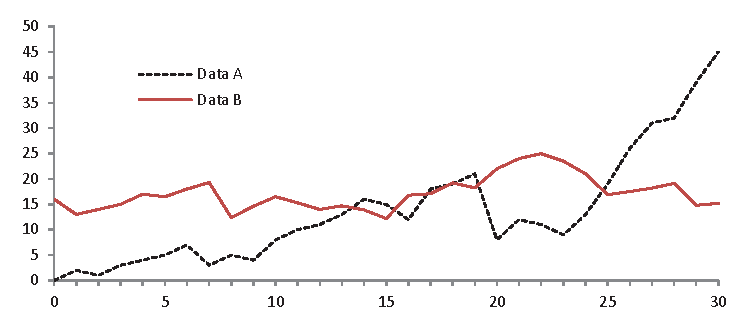
\includegraphics[width=\textwidth]{fig1.eps}
% \caption{A figure caption is always placed below the illustration.
% Please note that short captions are centered, while long ones are
% justified by the macro package automatically.} \label{fig1}
% \end{figure}
% 
% \begin{theorem}
% This is a sample theorem. The run-in heading is set in bold, while
% the following text appears in italics. Definitions, lemmas,
% propositions, and corollaries are styled the same way.
% \end{theorem}
% %
% % the environments 'definition', 'lemma', 'proposition', 'corollary',
% % 'remark', and 'example' are defined in the LLNCS documentclass as well.
% %
% \begin{proof}
% Proofs, examples, and remarks have the initial word in italics,
% while the following text appears in normal font.
% \end{proof}
% For citations of references, we prefer the use of square brackets
% and consecutive numbers. Citations using labels or the author/year
% convention are also acceptable. The following bibliography provides
% a sample reference list with entries for journal
% articles~\cite{ref_article1}, an LNCS chapter~\cite{ref_lncs1}, a
% book~\cite{ref_book1}, proceedings without editors~\cite{ref_proc1},
% and a homepage~\cite{ref_url1}. Multiple citations are grouped
% \cite{ref_article1,ref_lncs1,ref_book1},
% \cite{ref_article1,ref_book1,ref_proc1,ref_url1}.
%
% ---- Bibliography ----
%
% BibTeX users should specify bibliography style 'splncs04'.
% References will then be sorted and formatted in the correct style.
%
\bibliographystyle{splncs04}
\bibliography{main}
%
% \begin{thebibliography}{8}
% \bibitem{ref_article1}
% Author, F.: Article title. Journal \textbf{2}(5), 99--110 (2016)
% 
% \bibitem{ref_lncs1}
% Author, F., Author, S.: Title of a proceedings paper. In: Editor,
% F., Editor, S. (eds.) CONFERENCE 2016, LNCS, vol. 9999, pp. 1--13.
% Springer, Heidelberg (2016). \doi{10.10007/1234567890}
% 
% \bibitem{ref_book1}
% Author, F., Author, S., Author, T.: Book title. 2nd edn. Publisher,
% Location (1999)
% 
% \bibitem{ref_proc1}
% Author, A.-B.: Contribution title. In: 9th International Proceedings
% on Proceedings, pp. 1--2. Publisher, Location (2010)
% 
% \bibitem{ref_url1}
% LNCS Homepage, \url{http://www.springer.com/lncs}. Last accessed 4
% Oct 2017
% \end{thebibliography}

\blue{We solicit submissions in the form of regular research papers describing original scientific research results, including system development and case studies. Regular research papers should not exceed 18 pages in the Springer LNCS format, including bibliography and figures. This category encompasses both theoretical and implementation (also known as system descriptions) papers. In either case, submissions should clearly identify what has been accomplished and why it is significant. Submissions will be judged on the basis of significance, relevance, correctness, originality, and clarity. System descriptions papers should contain a link to a working system and will be judged on originality, usefulness, and design. In case of lack of space, proofs, experimental results, or any information supporting the technical results of the paper could be provided as an appendix or a link to a web page, but reviewers are not obliged to read them.}
\end{document}
